\subsection{Comparative study: MODIS cloud data}\label{sec:04-01:MODIS}

% \begin{itemize}
%     \item \red{Maybe I need to use the samples of the probability process to simulate from a Bernoulli distribution, like I did for the Chicago example (Poisson).}
% \end{itemize}

\begin{figure}[t!]
    \centering
    \includegraphics[width = \linewidth]{Images/MODIS_data.pdf}
     \caption[MODIS dataset: original image, and the subsample]{MODIS data. The original image (left panel) of the cloud, and an example of sub-sample of the original image (right panel) used as training data. The original image has 33750 pixels; the sub-sample has 2000 pixels. In the right panel, a blue background is chosen to make the ``No Cloud'' and the ``Cloud'' pixels easier to distinguish. 
     In this comparison study, we used 10 different training sets and averaged the results.}\label{fig:03-04-Modis1}
\end{figure}


We now compare the analysis of a real Bernoulli dataset as performed by the \texttt{R} packages \texttt{FRKv2}, \texttt{INLA} \citep{Lindgren_2015_R-INLA},  \texttt{spNNGP} \citep{Finley_2020_spNNGP}, \texttt{spBayes} \citep{Finley_2015_spBayes}, and \texttt{mgcv} \citep{Wood_2017_GAM:R}. 
% Before comparing the analysis of each package, we first briefly describe the data. 
The data is an image of a cloud taken by the Moderate Resolution Imaging Spectroradiometer (MODIS) instrument aboard the Aqua satellite \citep{MODIS_satelitte}. 
Data collected from the MODIS instrument has been used in several recent works; see, for instance, \cite{Sengupta_2016_MODIS} and  \cite{ZammitMangion_2020_Deep_compositional_spatial_model}.
For this comparative study, data pre-processing involved first coarsening the image from over 10 million pixels to a more manageable 33750 pixels, by creating a coarse 150 $\times$ 225 grid and computing the mean value of the response within each grid cell. 
Then, as the data provided by the MODIS instrument is continuous (measuring radiance), we applied a reasonable threshold to obtain a binary version of the data (i.e., cloud, or no-cloud).
The left panel of Figure \ref{fig:03-04-Modis1} displays the processed image of the cloud. 
% The image consists of regions that have no cloud cover (black), and regions that have cloud cover (white). 




\begin{figure}[t!]
    \centering
    \includegraphics[width = \linewidth]{Images/MODIS_pred_and_uncert.pdf}
     \caption{Point predictions and corresponding uncertainty quantification of predictions of the probability of cloud being present for each model used in the MODIS comparison study. }   
  \label{fig:MODIS:pred_and_uncert}
\end{figure}


\begin{figure}[t!]
    \centering
    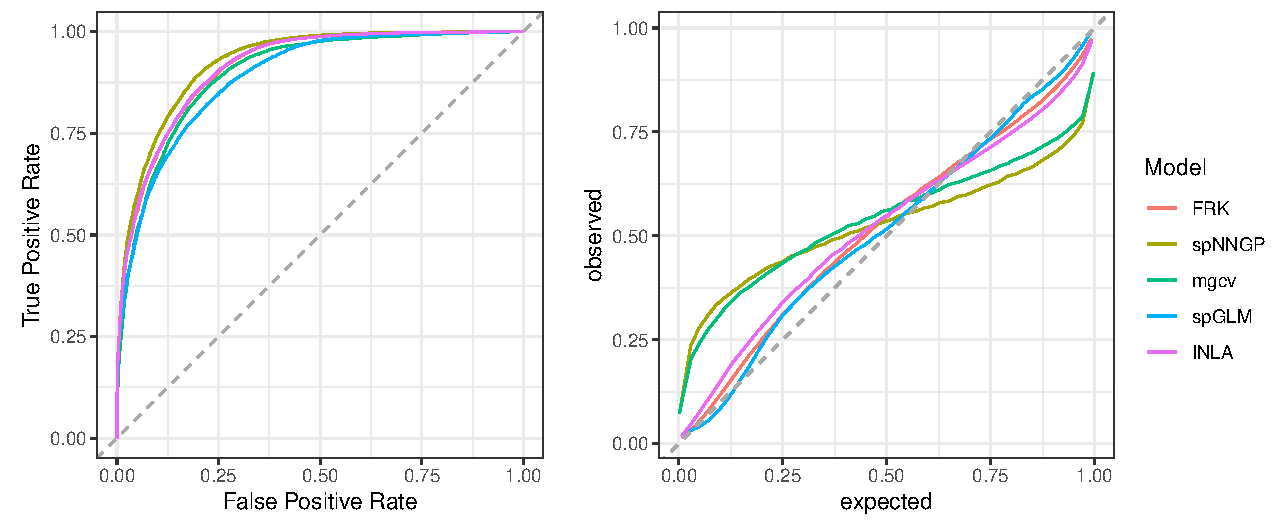
\includegraphics[width = \linewidth]{Images/ROC_and_KS.pdf}
    \caption{ROC curves, and observed vs. expected proportions of ones in each bin, for the training set displayed in Figure \ref{fig:03-04-Modis1}. (Left panel) ROC curves; models with better prediction have curves closer to the top left corner. (Right panel) Plot of the observed against expected proportions of ones in each bin; models with better prediction have curves closer to the identity line. 
    \red{(Not all lines visible in left panel due to overlapping.  Needs to be fixed somehow, at worst, indicate the problem in the caption. I think I should be able to fix it by setting the alpha parameter to be like 0.5. Probably also good to mention in the caption that there is significant overlap between FRK and INLA in the ROC curves. Also need to change the axis labels for the right plot; perhaps change to ``Expected proportion of ones'' and ``Observed proportion of ones''. )}}   
  \label{fig:MODIS:ROC_and_KS}
\end{figure}

% For this comparison study, we considered two types of sampling schemes for validation.
% The first is missing-at-random (MAR), whereby we randomly select a sub-sample of pixels to act as training data.
% Under the MAR sampling scheme, we randomly sampled 2000 pixels for training, leaving 31750 pixels for validation
% The second sampling scheme, which we refer to as missing-box (MB), involves excluding all pixels within a box for training, and using the box for validation. 
% \red{How big is the box, and how many pixel?}
% The centre panel and right panel of Figure \ref{fig:03-04-Modis1} displays an example of a training set under the MAR and MB sampling schemes, respectively. 
% To obtain reliable estimates of computational times and diagnostic scores, we repeated the experiment 10 times for each sampling scheme, and then averaged the results. 
% We compared the predictions from all the models in
% terms of the conventional Brier score \citep[sec 3.]{Gneiting_2007_scoring_rules},
% the posterior predictive expected Brier score (see Appendix \ref{app:ScoringRules}), the Kolmogorov-Smirnov statistic, and the area under the ROC curve (AUC). 
% These scoring rules are described in Appendix \ref{app:ScoringRules}. 

For this comparison study, the objective is to determine whether a given (partially unobserved) region has cloud cover or not.
To obtain a training- and test-set, we used a missing-at-random (MAR) sampling scheme, whereby we randomly select a sub-sample of 2000 pixels to act as training data, and use the remaining 31750 pixels as validation data.
The right panel of Figure \ref{fig:03-04-Modis1} displays an example of a training set under this sampling scheme. 
Using the training set in Figure \ref{fig:03-04-Modis1}, we generated point predictions and Highest Posterior Density (HPD) predictive intervals for each model; this is displayed in Figure \ref{fig:MODIS:pred_and_uncert}.



Each of the packages used in this comparison study require several modelling decisions, which must be made in a way that balances predictive performance and computational time. 
Some decisions are common to several packages packages; for instance, we chose the link function to be the standard logit link, and the number of predictive samples used for all packages is set 400 so that simulation error is consistent for all packages.
%%%% FRKv2
% For \texttt{FRKv2}, we chose \texttt{nres = 3}, which indicates three resolutions of spatial basis functions, and, for this spatial domain,  resulted in a total of 1248 basis functions.
% As discussed previously, when using a non-Gaussian data model, it is more computationally efficient to use the prior precision matrix formulation for the basis function random coefficients, which is indicated by setting \texttt{K\_type = "neighbour"} in \texttt{SRE()}.
For \texttt{FRKv2}, we used 1248 basis functions, and the prior precision matrix formulation for the basis function random coefficients.
%%%% INLA
For \texttt{INLA}, we set the number of basis functions to 3043.
Using \texttt{INLA} also requires specification of the prior distributions over the hyper-parameters, specifically, the range parameter, and the marginal standard deviation. 
% These priors are set using the arguments \texttt{prior.range} and \texttt{prior.sigma} within the function \texttt{inla.spde2.pcmatern()}. 
The pixels in this example are squares with unit dimensions; it is unlikely that the spatial range is smaller than the pixel size, so we specified a lower reasonable value of 1. 
We set a reasonable upper value for the marginal standard deviation to be three times the sample standard deviation (after adding 0.05 to data with a value of 0, subtracting 0.05 from data with a value of 1, and applying the logit link function). 
%%%% mgcv
For \texttt{mgcv}, 
%%%% spGLM
and \texttt{spGLM}, we used 250 and 81 knots, respectively,  
%%%% spNNGP
while we considered 10 neighbours at a time when using \texttt{spNNGP}.
%%%% spNNGP/spGLM
% Both \texttt{spNNGP} and \texttt{spGLM} use Markov chain Monte Carlo (MCMC), which typically requires more decisions to be made compared to \texttt{FRK}, \texttt{INLA}, and \texttt{mgcv}. 
Both \texttt{spNNGP} and \texttt{spGLM} use Markov chain Monte Carlo;  
at both training and test locations, we used 10000 total samples, a burn-in of 6000, and a thinning factor of 10 (hence, 400 approximately independent samples were produced at each location). 
For \texttt{spNNGP}, the tuning parameter was set to be 0.15, whilst it was set to 0.5 for \texttt{spGLM}; these values were chosen so that the acceptance rate was between 25\% and 50\%, as recommended by the package authors (the final acceptance rates were 32.94\% and \red{spGLM acceptance rate}). 
\texttt{spNNGP} allows users to specify the number of cores; in this analysis, we set this to 1, but note that the \texttt{spNNGP} authors stress that the algorithm benefits from multiple cores.
\red{I need to figure out how many cores to use. I also think I need to experiment with a different number of MCMC samples; perhaps 10,000 is too many, or a thinning factor of 10 is too great (these were just the numbers used by the examples in their papers). I think the spNNGP paper showed that about 18 cores is optimal. Maybe if I re-do it on my Linux, I'll just set it to the maximum (8).}






We compared the predictions from all models in terms of the conventional Brier score \citep[sec.~3]{Gneiting_2007_scoring_rules}, the posterior predictive expected (PPE) Brier score, the Kolmogorov-Smirnov (KS) statistic and its associated p-value, and the area under the receiver operating characteristic (ROC) curve (AUC); these scoring rules are detailed in Appendix \ref{app:ScoringRules}. 
The conventional Brier score uses a point-prediction of the probability of cloud, and quantifies how close this prediction is to the observed data.
The PPE Brier score assesses how close a predictive \textit{distribution} is to the observed value, and involves computing the expectation of the conventional Brier score with respect to the posterior distribution of the probability process.
The principle underlying our use of the KS statistic is that, globally, predictive samples of the probability process $\pi(\cdot)$ which have a value of $\pi_0$ should, on average, be associated with cloud pixels $\pi_0\times 100\%$ of the time, and be associated with non-cloud pixels $(1- \pi_0)\times 100\%$ of the time. This notion is formalised in Appendix \ref{app:ScoringRules:KS-statistic}.
Each of these diagnostic scores are negatively oriented, that is, low scores are preferred. 
To obtain reliable estimates of computational times and diagnostic scores, we repeated the experiment 10 times (i.e., with 10 different randomly-sampled training sets), and then averaged the results; these results are reported in Table \ref{tab:summary_of_analyses}. 
\texttt{FRKv2}, whilst not being the highest performer in any category, is consistently close to the best.
\red{Need more comparisons, and to spell out the results for the reader.}

\texttt{spNNGP} gets things right in expectation (hence, the favourable conventional Brier score), but less so in predeictive variance (hence the worse results in terms of PPE Brier score and KS).


In Figure \ref{fig:MODIS:ROC_and_KS}, we present the ROC curves for each package, as well as the plot of observed against expected proportion of ones in each bin (see Appendix \ref{app:ScoringRules}). 
The latter plot suggests that \texttt{FRKv2} is correctly quantifying the prediction uncertainty.
\red{Need a  better discussion. Things which need to be discussed:
Differences that come out between the Brier score and its posterior predictive version, the 0s of the KS statistics, and computation time, and anything else interesting you may think of. 
Spelling out what the results mean in the main text is also important (and what you conclude from them).}

\red{One thing I can point out is that the predictive performance of FRK is very similar to that of \texttt{INLA}, but the computational time is much less (well, lets see how things go with my Linux; as they currently are, the timings are quite similar).}


\begin{table}
    \centering
    \caption{Averaged diagnostic results for the MODIS comparison study. Highest performers for a given diagnostic score are boldfaced. \red{Perhaps I should re-do this on my Linux computer, as it is easier to quote the specs (and be sure that they are consistent) compared to the HPC. I should also signify in the table how many cores are used (perhaps the table caption if the number of cores is the same for all packages).}}
    \label{tab:summary_of_analyses}
    \begin{tabular}{lcccccc}
    \hline\hline
     Method  & Con. Brier score & PPE Brier score & AUC & KS & KS p-value & Comp. time (secs.) \\[3pt]\hline
    \texttt{FRKv2}  & 0.114 & 0.140 & 0.920 & 0.078 & 0.102  & 103.26\\
    \texttt{spNNGP}   & \textbf{0.106} & {0.170} & \textbf{0.928} & 0.286 & {0.000} & 303.14\\
     \texttt{mgcv}     & {0.125} & {0.162} & {0.902} & 0.215 & {0.000} & \textbf{20.89} \\
     \texttt{spGLM}    & {0.132} & {0.138} & {0.892} & 0.055 & \textbf{0.5385} & 297.97\\
     \texttt{INLA}     & {0.114} & \textbf{0.135} & {0.920} & 0.101 & {0.014} & 157.58\\
    \hline
  \end{tabular}
\end{table}